\begingroup
\setlength{\abovedisplayskip}{6pt}
\setlength{\belowdisplayskip}{6pt}
\setlength{\abovedisplayshortskip}{4pt}
\setlength{\belowdisplayshortskip}{4pt}
\setlength{\intextsep}{6pt}

The given initial conditions are $u(0)=u_0=13\ \mathrm{mm}$ and $\dot{u}(0)=\dot{u}_0=0$. The natural frequency is specified by $f_n=6.25\ \mathrm{Hz}$.

\textbf{B.5.1. Input data.}

{ % do not increment counter
\begin{center}\small\begin{tabular}{@{}lrl@{}}
\toprule\noalign{}
Quantity & Value & Unit \\
\midrule\noalign{}
$f_n$ & 6.25 & Hz \\
$u_0$ & 13.0 & mm \\
$\dot{u}_0$ & 0 & mm/s \\
$t$ & $0$--$3$ & s \\
\bottomrule\end{tabular}\end{center}
}

\textbf{B.5.2. Natural frequency.}

The frequency in hertz is converted to angular frequency by multiplying by $2\pi$.

\[
\omega_n=2\pi f_n=2\pi(6.25)=39.2699\ \mathrm{rad/s}.
\]

\[
\boxed{\omega_n=39.27\ \mathrm{rad/s}}
\qquad\text{(B.5.2)}
\]

\textbf{B.5.3. Overdamped response with $\zeta=2.3$.}

For free vibration, the characteristic equation is

\[
s^2+2\zeta\omega_n s+\omega_n^2=0.
\]

\textbf{(a) Roots.} Since $\zeta>1$, the discriminant is positive and the two roots are real. Letting $s_1$ denote the faster root and $s_2$ the slower root gives

\[
s_1=-\left(\zeta+\sqrt{\zeta^2-1}\right)\omega_n,
\qquad
s_2=-\left(\zeta-\sqrt{\zeta^2-1}\right)\omega_n.
\]

\[
\boxed{
s_1=-\left(\zeta+\sqrt{\zeta^2-1}\right)\omega_n,
\qquad
s_2=-\left(\zeta-\sqrt{\zeta^2-1}\right)\omega_n
}
\qquad\text{(B.5.3.a)}
\]

\textbf{(b) General solution.} Each real root produces an exponential partial solution. Their linear combination is

\[
\boxed{u(t)=C_1e^{s_1t}+C_2e^{s_2t}}
\qquad\text{(B.5.3.b)}
\]

\textbf{(c) Initial-condition constants.} Evaluating the response at $t=0$ gives $C_1+C_2=u_0$. Differentiating first and then evaluating at $t=0$ gives $s_1C_1+s_2C_2=\dot{u}_0$. Solving these two equations yields

\[
\boxed{
C_1=\frac{\dot{u}_0-s_2u_0}{s_1-s_2},
\qquad
C_2=\frac{s_1u_0-\dot{u}_0}{s_1-s_2}
}
\qquad\text{(B.5.3.c)}
\]

\textbf{(d) Numerical values.} For $\zeta=2.3$,

\[
\sqrt{\zeta^2-1}=\sqrt{2.3^2-1}=2.07123.
\]

Substitution into the root expressions gives

\[
\begin{aligned}
s_1&=-(2.3+2.07123)(39.2699)=-171.658\ \mathrm{s^{-1}},\\
s_2&=-(2.3-2.07123)(39.2699)=-8.98372\ \mathrm{s^{-1}}.
\end{aligned}
\]

Using $u_0=13\ \mathrm{mm}$ and $\dot{u}_0=0$ in the constant expressions gives

\[
C_1=\frac{0-(-8.98372)(13)}{-171.658-(-8.98372)}=-0.71793\ \mathrm{mm},
\]

\[
C_2=\frac{(-171.658)(13)-0}{-171.658-(-8.98372)}=13.71793\ \mathrm{mm}.
\]

\[
\boxed{
\begin{aligned}
s_1&=-171.658\ \mathrm{s^{-1}},&
s_2&=-8.98372\ \mathrm{s^{-1}},\\
C_1&=-0.71793\ \mathrm{mm},&
C_2&=13.71793\ \mathrm{mm}
\end{aligned}}
\qquad\text{(B.5.3.d)}
\]

Therefore, the overdamped displacement is

\[
u_{\mathrm{OD}}(t)=-0.71793e^{-171.658t}+13.71793e^{-8.98372t}\ \mathrm{mm}.
\]

\textbf{(e) Overdamped plot.} The response is plotted over the required interval $0\leq t\leq3\ \mathrm{s}$.

\begin{figure}[H]
\centering
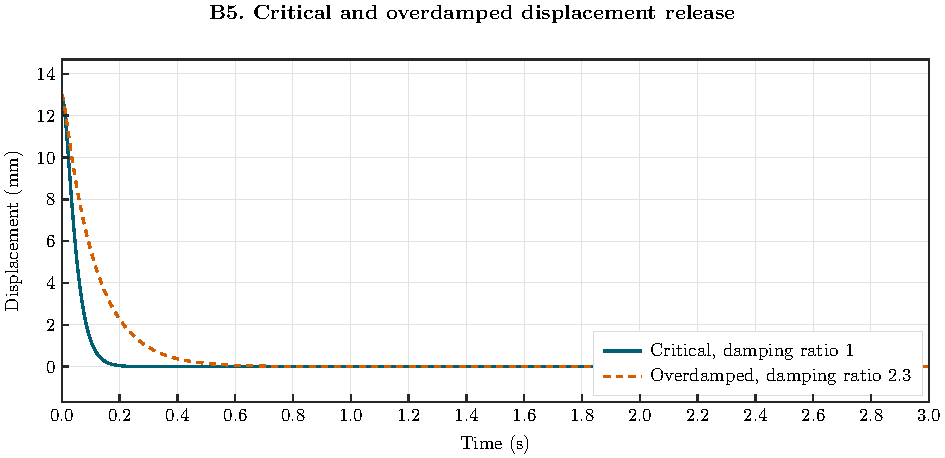
\includegraphics[width=0.95\linewidth,height=0.30\textheight,keepaspectratio,alt={B.5.3.e. Overdamped and critical responses over the required three-second interval.}]{figures/generated/solutions/B5.pdf}
\caption{B.5.3.e. Overdamped and critical responses over $0\leq t\leq3\ \mathrm{s}$.}
\end{figure}

\textbf{B.5.4. Critically damped response with $\zeta=1$.}

\textbf{(a) Partial solutions.} At $\zeta=1$, the two roots merge into the repeated root $s=-\omega_n$. One solution is the exponential associated with that root. A second independent solution is obtained by multiplying the exponential by $t$.

\[
\boxed{u_1(t)=e^{-\omega_nt},
\qquad
u_2(t)=te^{-\omega_nt}}
\qquad\text{(B.5.4.a)}
\]

\textbf{(b) Complete solution.} The complete response is the linear combination of the two independent partial solutions.

\[
\boxed{u(t)=\left(C_1+C_2t\right)e^{-\omega_nt}}
\qquad\text{(B.5.4.b)}
\]

\textbf{(c) Initial-condition constants.} At $t=0$, the displacement condition gives $C_1=u_0$. Differentiating the complete solution gives

\[
\dot{u}(t)=\left[C_2-\omega_n(C_1+C_2t)\right]e^{-\omega_nt}.
\]

Evaluating at $t=0$ gives $\dot{u}_0=C_2-\omega_nC_1$. Therefore,

\[
\boxed{C_1=u_0,
\qquad
C_2=\dot{u}_0+\omega_nu_0}
\qquad\text{(B.5.4.c)}
\]

\textbf{(d) Numerical values.} The constants are

\[
C_1=13.000\ \mathrm{mm},
\qquad
C_2=0+(39.2699)(13)=510.509\ \mathrm{mm/s}.
\]

\[
\boxed{C_1=13.00\ \mathrm{mm},
\qquad
C_2=510.51\ \mathrm{mm/s}}
\qquad\text{(B.5.4.d)}
\]

The critically damped displacement is consequently

\[
u_{\mathrm{CD}}(t)=\left(13+510.509t\right)e^{-39.2699t}\ \mathrm{mm}.
\]

\textbf{(e) Critically damped plot.} The shorter time view makes the difference between the two nonoscillatory responses visible near the initial displacement.

\begin{figure}[H]
\centering
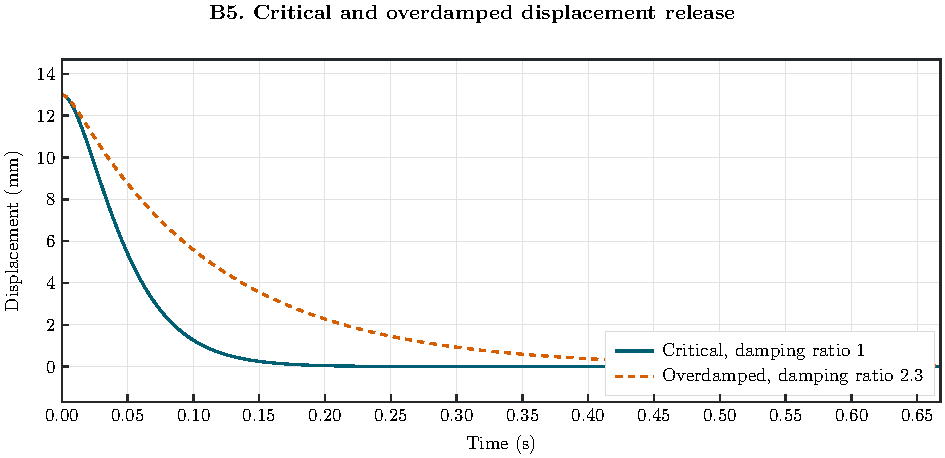
\includegraphics[width=0.95\linewidth,height=0.30\textheight,keepaspectratio,alt={B.5.4.e. Detailed comparison of critically damped and overdamped responses.}]{figures/generated/solutions/B5_detail.pdf}
\caption{B.5.4.e. Detailed comparison of the critically damped and overdamped responses.}
\end{figure}

\textbf{B.5.5. Verification of the critical-damping ODE.}

At critical damping, $c=2m\omega_n$ and $k=m\omega_n^2$. Substitution into $m\ddot{u}+c\dot{u}+ku=0$, followed by division by $m$, gives

\[
\ddot{u}+2\omega_n\dot{u}+\omega_n^2u=0.
\]

For $u_1=e^{-\omega_nt}$, differentiation gives $\dot{u}_1=-\omega_nu_1$ and $\ddot{u}_1=\omega_n^2u_1$. Substitution gives

\[
\ddot{u}_1+2\omega_n\dot{u}_1+\omega_n^2u_1
=\omega_n^2u_1-2\omega_n^2u_1+\omega_n^2u_1=0.
\]

For $u_2=te^{-\omega_nt}$, the first two derivatives are

\[
\dot{u}_2=(1-\omega_nt)e^{-\omega_nt},
\qquad
\ddot{u}_2=(\omega_n^2t-2\omega_n)e^{-\omega_nt}.
\]

Substitution into the ODE gives

\[
\begin{aligned}
\ddot{u}_2+2\omega_n\dot{u}_2+\omega_n^2u_2
&=(\omega_n^2t-2\omega_n)e^{-\omega_nt}
 +2\omega_n(1-\omega_nt)e^{-\omega_nt}
 +\omega_n^2te^{-\omega_nt}\\
&=0.
\end{aligned}
\]

Both partial solutions satisfy the critical-damping ODE, so their linear combination is also a solution.

\textbf{B.5.6. Critical versus overdamped design.}

Both designs return to equilibrium without oscillation. Critical damping has the repeated decay rate $-\omega_n$, so it gives the fastest nonoscillatory return for the specified $\omega_n$ and initial conditions. Its main disadvantage is that the damping must be tuned close to the critical value. Changes in mass, stiffness, or damper properties move the system away from that condition.

For $\zeta=2.3$, the overdamped response contains a fast rate of $-171.658\ \mathrm{s^{-1}}$ and a slow rate of $-8.98372\ \mathrm{s^{-1}}$. The fast exponential has a negative coefficient, so that term increases toward zero as it decays. The derivatives of the two terms cancel at release to give the specified zero initial velocity. For these initial conditions, the critically damped response returns faster both initially and at late times; the slow overdamped root controls the long tail. For example, at \(t=0.010\ \mathrm{s}\), the critical response is \(12.23\ \mathrm{mm}\), while the overdamped response is \(12.41\ \mathrm{mm}\). Overdamping can therefore provide more tolerance against crossing into oscillatory behavior, but it sacrifices response speed and can increase damper forces during rapid motion. A race-car suspension must balance these effects with tire contact, road inputs, suspension travel, and damper-force limits.

\clearpage
\matlabcaption{MATLAB script for the B.5 overdamped and critically damped response plots.}

\begin{center}
\begin{matlabcode}
fn = 6.25; u0 = 13; v0 = 0; z = 2.3;
t = linspace(0,3,2000); wn = 2*pi*fn;

q = sqrt(z^2-1); s1 = -(z+q)*wn; s2 = -(z-q)*wn;
C1 = (v0-s2*u0)/(s1-s2); C2 = (s1*u0-v0)/(s1-s2);
uOD = C1*exp(s1*t)+C2*exp(s2*t);
uCD = (u0+(v0+wn*u0)*t).*exp(-wn*t);

plot(t,uCD,'Color',[0 .427 .459],'LineWidth',1.5); hold on
plot(t,uOD,'--','Color',[.776 .365 0],'LineWidth',1.5)
xlabel('Time (s)'); ylabel('Displacement (mm)'); grid on
legend('Critical, zeta = 1','Overdamped, zeta = 2.3')
\end{matlabcode}
\end{center}

\endgroup
